% \documentclass[11pt,a4paper,twoside,extrafontsizes]{memoir}

\renewcommand*{\baselinestretch}{1.025}
\isopage
\checkandfixthelayout

\newif\iftdkoneside
\tdkonesidefalse

%%% Local Variables:
%%% mode: latex
%%% TeX-master: "../main"
%%% End:

% We actually use `twoside` in oneside mode to avoid renumbering pages.
\documentclass[11pt,a4paper,twoside,extrafontsizes]{memoir}

\renewcommand*{\baselinestretch}{1.04}
\isopage
\setlrmargins{*}{*}{1}
\checkandfixthelayout

\newif\iftdkoneside
\tdkonesidetrue

%%% Local Variables:
%%% mode: latex
%%% TeX-master: "../main"
%%% End:


\usepackage{include/tdk}


%
% General
%

\DeclareMathOperator*{\argmin}{arg\,min}
\DeclareMathOperator*{\argmax}{arg\,max}
\newcommand*{\dd}{\mathrm{d}}
\newcommand*{\T}{\mathrm{T}}
\newcommand*{\QED}{\hfill $\square$}
\newcommand*{\vecarrow}{}\let\vecarrow\vec
\renewcommand*{\vec}[1]{\bm{\mathrm{#1}}}

%
% Numbers
%

\newcommand*{\RR}{\mathbb{R}} % Reals
\newcommand*{\RRpos}{\RR^{+}} % Positiver reals
\newcommand*{\QQ}{\mathbb{Q}} % Rationals
\newcommand*{\ZZ}{\mathbb{Z}} % Whole numbers
\newcommand*{\NN}{\mathbb{N}} % Naturals
\newcommand*{\NNpos}{\NN^{+}} % Positive whole numbers

%
% Disjoint unions
%

% http://tex.stackexchange.com/a/52673/8744
\makeatletter
\def\moverlay{\mathpalette\mov@rlay}
\def\mov@rlay#1#2{\leavevmode\vtop{%
   \baselineskip\z@skip \lineskiplimit-\maxdimen
   \ialign{\hfil$\m@th#1##$\hfil\cr#2\crcr}}}
\newcommand{\charfusion}[3][\mathord]{
    #1{\ifx#1\mathop\vphantom{#2}\fi
        \mathpalette\mov@rlay{#2\cr#3}
      }
    \ifx#1\mathop\expandafter\displaylimits\fi}
\makeatother

\newcommand*{\cupdot}{\charfusion[\mathbin]{\cup}{\cdot}}
\newcommand*{\bigcupdot}{\charfusion[\mathop]{\bigcup}{\cdot}}

%
% Probability
%

\let\Pr\relax
\DeclareMathOperator{\Pr}{\mathbb{P}}
\DeclareMathOperator{\Ex}{\mathbb{E}}

%
% Hipergraphs
%

\newcommand*{\HH}{\mathcal{H}}
\newcommand*{\EE}{\mathcal{E}}
\newcommand*{\GG}{\mathcal{G}}
\newcommand*{\chromatic}{\chi}
\newcommand*{\weakChromatic}{\chi_{\textrm{gyenge}}}
\newcommand*{\strongChromatic}{\chi_{\textrm{erős}}}
\newcommand*{\edgeChromatic}{\chi_{e}}

%
% Sets, Families of sets
%

\renewcommand*{\AA}{\mathcal{A}}


%%% Local Variables:
%%% mode: latex
%%% TeX-master: "../main"
%%% End:


\newcommand*{\authors}{Szerzők}
\newcommand*{\authori}{Balogh László}
\newcommand*{\authorii}{Hegyi Bálint}
\newcommand*{\authoriii}{Marussy Kristóf}
\newcommand*{\authoriv}{Csala Tamás}

\newcommand*{\lecturer}{Előadó}
\newcommand*{\lectureri}{Dr.~Simonyi Gábor}

\newcommand*{\semester}{2016/2017.~tavaszi félév}

\title{Gráfok, hipergráfok és alkalmazásaik}
\newcommand*{\titlepagetitle}{Gráfok, hipergráfok\\és alkalmazásaik}
\author{\authori, \authorii, \authoriii, \authoriv}

\hypersetup{
  pdftitle={\thetitle},
  pdfauthor={\theauthor}
}

%%% Local Variables:
%%% mode: latex
%%% TeX-master: "../main"
%%% End:


\bibliography{references}

\begin{document}

\frontmatter

\thispagestyle{plain}

\cleartorecto
\thispagestyle{empty}

\begin{tikzpicture}[overlay,remember picture]
  \node at (current page.center) [yshift=1cm] {%
    \begin{minipage}{\textwidth}

      \centering

      
\includegraphics[width=7cm]{include/figures/bme_logo}
      \vspace{0.3cm}

      \bme \\
      \vik \\
      \bmemit \\
      \vspace{3.5cm}

      {\Large \authori \par}
      \vspace{0.5cm}

      {\Huge\sffamily\bfseries \titlepagetitle \par}
      \vspace{1cm}

      {\large \vikdoctype \par}
      \vspace{3.5cm}

      {\Large 
        \advisors: \\ \vspace{0.3cm}
        \advisori \\
        \advisorii \\
        \advisoriii\par}

      \vspace{1.5cm}
      {\large \viktdklocation, \viktdkyear\par}

    \end{minipage}};
\end{tikzpicture}

\cleardoublepage

%%% Local Variables:
%%% mode: latex
%%% TeX-master: "../main"
%%% End:


\tableofcontents

\mainmatter

\chapter{Baranyai tétele}

% \begin{dfn}
%   A $\GG$ gráfban egy $\HH$ részgráfot \emph{k-faktor}nak nevezünk, ha $\HH$ k-reguláris (vagyis $\HH$ minden csúcsának k a fokszáma) és feszítő részgráf ($\HH$ tartalmazza $\GG$ összes csúcsát).
% \end{dfn}

% A teljes párosítás egy 1-faktor.

% \begin{dfn}
%   Egy gráf éleinek particíóját k-faktorokba \emph{k-faktorizációnak nevezzük}. Ha egy gráfnak létezik \emph{k-faktorizációja}, akkor azt mondjuk, hogy \emph{k-faktorizálható}.
% \end{dfn}

% Az 1-faktorizációnak fontos szerepe van például sakkversenyek szervezésekor. Ha egy gráfban a csúcspontok a versenyzőket, az élek pedig lebonyolítandó játszmákat jelölik, akkor egy ilyen gráfnak az 1-faktorizációja egy olyan összeállítást ad meg, ahol egy faktor egy fordulónak felel meg, minden fordulóban minden játékos játszik, és semelyik pár sem játszik többször egymás ellen.

% \begin{thm}
%   Tetszőleges pozitív, páros $n$-re a $K_{n}$, az $n$-csúcsú teljes gráf 1-faktorizálható.
% \end{thm}

% A tétel legegyszerűbb bizonyítása a következő: $i = 1 , 2 , \dots , n - 1$ esetén az $i$-edik faktor álljon a $(0,~i)$ élből és az $(i-j , i+j) (mod~n - 1)$ élekből, ahol $j = 1 , 2 , \dots , \frac{n}{2} - 1$. A $K_8$ gráf esetén ez a konstrukció \aref{fig:faktorizacio}. ábrán látható.

% \includefigure[width=\textwidth]{faktorizacio}{A $K_8$ egy lehetséges egy faktorizációja}

\begin{thm} Baranyai-tétel:
  Minden $r|n$ viszonyt teljesítő $r,n$ párosra a $K^{r}_{n}$, az $r$-uniform $n$-csúcsú teljes hipergráf 1-faktorizálható.
\end{thm}

Egy ezzel ekvivalens tétel:
\begin{thm}
  Minden $r|n$ és $1 \leq k \leq n$ viszonyt teljesítő $r,n,k$ értékekre a $\{1, 2, \dots, k\}$ halmaznak (ezt a halmazt jelölje $[k]$ a későbbiekben) van $M = \binom{n-1}{r-1}$ db olyan partíciója legfeljebb r méretű halmazokra, hogy minden partícióban az $\emptyset$-t is megengedve $m = \frac{n}{r}$ osztály van, és $\forall s \subseteq [k]$ részhalmaz pontosan $\binom{n-k}{r-|s|}$ partícióban fordul elő.
\end{thm}

Megjegyzések:
\begin{itemize}
  \item Ez a Baranyai tételhez hasonló állítást mond ki, de csak az első k elem lehetséges értékeinek particionálásra.
  \item a k=n eset visszaadja a Baranyai tételt, hiszen $\binom{0}{r-|s|}$ értéke egy, ha $s=n$ és nulla, ha $s \neq n$. Azaz az alaphalmaznak létezik $M$ db partíciója $m$ részre, úgy, hogy minden partíció pontosan n elemet tartalmaz (vagyis a partíciók az összes elemet tartalmazzák).
  \item Ennek a tételnek az a jelentősége, hogy indukcióval könnyen bizonyítható, és ez a bizonyítás a Baranyai tételt is igazolja.
\end{itemize}

Bizonyítás (Ekvivalens tétel):
\begin{itemize}
  \item $k=0$-ra $\forall$ minden partícióosztály üres, és $\binom{n}{r}$-szer fordul elő. Ez megegyezik a tétel állításával.

  \item Lemma az indukciós lépéshez:
  Legyen $A = \{a_{i,j}\}, i \in \{1, \dots, t\}, j \in \{1, \dots, h\}$ olyan mátrix, amiben a sor és oszlopösszegek egész számok.

  Ekkor $\exists$ olyan $B = \{b_{i,j}\}, i \in \{1, \dots, t\}, j \in \{1, \dots, h\}$ mátrix, ahol $b_{i,j}~=~\lceil a_{i,j} \rceil$ vagy $b_{i,j}~=~\lfloor a_{i,j} \rfloor$, és minden sor és oszlopösszeg megegyezik az A-belivel.

  Biz: Ha A minden eleme egész, akkor készen vagyunk. Különben induljunk ki egy nem egész elemből. Az egész sorösszeg miatt lesz a sorában legalább egy másik nem egész elem, aminek az oszlopában szintén lesz egy nem egész elem, stb. A véges sok elem miatt előbb-utóbb elérünk egy olyan elemhez, ahol egyszer már jártunk. Az útvonalban felhasznált elemnek lesz olyan részhalmaza, ami egy páros sok elemből álló kört alkot (a vízszintes és függőleges mozgások váltakozása miatt). Legyen $\delta$ az a legkisebb abszolút értékű szám, amit az egyik elemhez hozzá kell adni, hogy egész legyen. A kör mentén felváltva $+\delta$-val és $-\delta$-val módosítsuk az elemeket, úgy, hogy az egészhez legközelebbi elem egésszé váljon. Így legalább eggyel több egész szám lesz a mátrixban, és a sor- és oszlopösszegek nem változnak. Ezt az algoritmust ismételjük, amíg minden elem egész nem lesz.

  \item Indukciós lépés $k$-ra:
  Tekintsük azt a mátrixot, aminek a sorai a $k$-ra vonatkozó állítást teljesítő partíciók, oszlopai $[k]$ részhalmazai és az $i$-edik partíció $s$-hez tartozó oszlopában szereplő érték az $\frac{\binom{n-k-1}{r-|s|-1}}{\binom{n-k}{r-s}} = \frac{r-|s|}{n-k}$, ha $s$ megjelenik az $i$-edik partícióban partícióosztályként (és $s \neq \emptyset$), nulla egyébként. $S = \emptyset$ esetén is ugyanígy járunk el, csak az értéket még felszorozzuk az $\emptyset$ multiplicitásával.

  Erre a mátrixra alkalmazzuk az előbb ismertetett lemmát. Erre egy példa \aref{fig:baranyai} ábrán látható.

  Vegyük észre, hogy kezdetben minden sörösszeg egy. Ha $R$ jelöli az adott sorhoz tartozó partíciót:
  \[\sum_{s \in R} \frac{r-|s|}{n-k} = \frac{\frac{n}{r} \cdot r - \sum_{s \in R} |s|}{n - k} = \frac{n-k}{n-k} = 1\]

  Tehát a kapott egész értékű mátrix minden sorában pontosan egy egyes lesz, aminek a jelentése, hogy az adott sorhoz tartozó partícióban az egyes oszlopának megfelelő partícióosztályt kell bővíteni a $k+1$ nevű elemmel.

  Továbbá minden oszlopban (az $\emptyset$-et kivéve) a nem nulla elemek értéke $\frac{\binom{n-k-1}{r-|s|-1}}{\binom{n-k}{r-s}}$ a mátrix konstrukciója miatt, és nem nulla elemből pontosan $\binom{n-k}{r-s}$ db van (az indukciós feltevés miatt). Ezen számok összege (a szorzatuk) $\binom{n-k-1}{r-|s|-1}$. Vagyis az $k+1$ nevű elem felvétele után a $k'= k+1$ és $s' = s \cup \{k+1\}$-re igaz, hogy $s'$ előfordulásainak száma $\binom{n-k'}{r-|s'|}$

  \includefigure[width=\textwidth]{baranyai}{Az indukciós lépés $k=2$-ről indulva}
\end{itemize}

\QED

%%% Local Variables:
%%% mode: latex
%%% TeX-master: "../main"
%%% End:

\chapter{Sperner tétel és LYM egyenlőtlenség}

\begin{dfn}
  Egy $\AA \subseteq 2^{[n]}$ \emph{Sperner rendszer}, ha $\forall A, B \in \AA: A \not \subseteq B, B \not \subseteq A$, ha $A \neq B$.
\end{dfn}

\begin{thm} Sperner-tétel:
  Ha $\AA$ egy Sperner rendszer, akkor $|\AA| \leq \binom{n}{\lfloor \frac{n}{2} \rfloor}$
\end{thm}

Bizonyítás (dupla leszámlálással):

\begin{notation}
  $S_n$ jelentse az n elemű szimmetrikus csoportot, azaz az első n elem permutációját.
\end{notation}

Tekintsük az olyan $(A, \sigma)$ párokat, ahol $A \in \AA$ és $\sigma \in S_n$, $\sigma = \sigma(1)\sigma(2) \dots \sigma(n)$ és $A = \sigma(1)\sigma(2) \dots \sigma(k)$, valamely k-ra (k=|A|). Azaz az $A$ ``párja'' $\sigma$-nak azt jelenti, hogy az $A$ eleminek létezik olyan sorrendje, hogy az így kapott sorozat prefixe a $\sigma$-nak. Az ilyen párok halmazát jelöljük $T$-vel.

\medskip

Egyrészt rögzített $\sigma \in S_n$-re legfeljebb egy $A \in \AA$ lehet, ami az ő párja, mert ha több is lenne, akkor azok tartalmaznák egymást, ami a Sperner-rendszer feltétele miatt ellentmondás. Emiatt $T$-nek legfeljebb annyi eleme lehet, ahány különböző értéket a $\sigma$ felvehet:
\[|T| \leq |S_n| = n!.\]

Másrészt rögzített $A \in \AA$ esetén a hozzá párba állítható $\sigma$-k számát csak az $A$-beli elemek sorrendje, és az $A$-ban nem szereplő, a $\sigma$ első $|A|$ eleme után folytatódó elemek sorrendje befolyásolja, vagyis a T-beli elemek száma:
\[|T| = \sum_{A \in \AA} |A|! (n-|A|)! \geq |\AA| \lfloor \frac{n}{2} \rfloor ! \lceil \frac{n}{2} \rceil !.\]

T elemszámára két összefüggést kaptunk, ezeket összevetve:
\begin{align}
  |\AA| \lfloor \frac{n}{2} \rfloor ! \lceil \frac{n}{2} \rceil ! &\leq |T| \leq n! \\
  |\AA| &\leq \frac{n!}{\lfloor \frac{n}{2} \rfloor ! \lceil \frac{n}{2} \rceil !}\\
  |\AA| &\leq \binom{n}{\lfloor \frac{n}{2} \rfloor}.
\end{align}

\QED

\begin{thm} LYM-tétel:
  Ha $\AA \subseteq 2^{[n]}$ Sperner rendszer és $f_k$ jelöli minden $k$-ra az $\AA$-ban lévő pontosan $k$ elemű halmazok számát, akkor $\sum_{k=0}^{n} \frac{f_k}{\binom{n}{k}} \leq 1$
\end{thm}

Biz (előző alapján):

\[\sum_{A \in \AA} |A|! \cdot (n - |A|)! \leq n!\]

\[\sum_{A \in \AA} \frac{1}{\frac{n!}{|A|! \cdot (n - |A|)!}} \leq 1\]

\[\sum_{A \in \AA} \frac{1}{\binom{n}{|A|}} \leq 1\]

\[\sum_{k = 0}^{n} \frac{f_k}{\binom{n}{k}} \leq 1\]

\QED

\begin{dfn} Lánc:
  $L \subseteq 2^{[n]}$, amire $B, B' \in L \Rightarrow B \subseteq B'$ vagy $B' \subseteq B$
\end{dfn}

Sperner-tétel másik bizonyítása:
Azt mutatjuk meg, hogy $2^{[n]}$ particionálható $\binom{n}{\lfloor \frac{n}{2}\rfloor}$ láncra.

Definiáljuk $\binom{[n]}{k}$ és $\binom{[n]}{k-1}$ között azt a $\GG$ páros gráfot, ahol az élek tartalmazást jelentenek: $A \in \binom{[n]}{k}$ és $B \in \binom{[n]}{k-1}$-re $AB$ él, pontosan akkor, ha $B \subset A$.

\begin{prop}
  Ha $k > \frac{n}{2}$ akkor $\GG$-ben $\exists \binom{[n]}{k}$-t fedő párosítás, ha pedig $k \leq \frac{n}{2}$ akkor $\exists \binom{[n]}{k-1}$-et fedő párosítás.
\end{prop}

Állítás biz ($k > \frac{n}{2}$ eset):
Legyen $x \subseteq \binom{[n]}{k}$. $\forall A \in x$-nek pontosan $k$ szomszédja van $\binom{[n]}{k-1}$-ben. Tehát $x$ és $N(x)$ között $|X| \cdot k$ él fut. $\forall B \in N(x)$-nek $n-k+1$ szomszédja van $\binom{[n]}{k}$-ban (ezek lehetnek $x$-ben és $x$-en kívül is) $\Rightarrow$ Az $x$ és $N(x)$ közötti élek száma $\leq |N(x)| \cdot (n-k+1)$.

Tehát $|x| \cdot k \leq |N(x)|(n-k+1)$, azaz $|N(x)| \geq |x| \frac{k}{n-k-1} \geq |x|$, ha $k > \frac{n}{2}$, mert $k > \frac{n}{2}$-re $k \geq n-k+1$.

\medskip

Állítás biz ($k \geq \frac{n}{2}$ eset):
Hasonlóan, $|x| (n-k+1) \leq |N(x)| \cdot k$, azaz $|N(x)| \geq |x| \frac{n-k+1}{k} \geq |x|$, mert $k \geq \frac{n}{2}$-re $n-k+1 \geq k$.

\medskip

A kapott párosítások felhasználásával adódik a láncokra való felbontás. Mivel egy Sperner rendszerben nem lehet több elem egyetlen láncból, ha $\AA$ Sperner rendszer, akkor $|\AA| \leq \binom{n}{\lfloor \frac{n}{2} \rfloor}$, azaz a láncfelbontásbeli láncok száma.

\QED

\chapter{Bollobás egyenlőtlenség}

\chapter{Ahlswede-Zhang azonosság}

\chapter{Kolexikografikus rendezés. Pozitív egészek felírása r-binomiális alakban, a felírás egyértelműsége.}

\begin{dfn} Egy halmazrendszer árnyéka:
  $\partial \FF = \{B \in \binom{[n]}{r-1}: \exists F \in \FF, B \subseteq F\}$
\end{dfn}

Probléma: Ha $\FF \subseteq \binom{[n]}{r}$ és egy fix $m$-re $|\FF|=m$, akkor hogyan kell megválasztani $\FF$ elemeit, hogy $|\partial \FF|$ minimális legyen?

\vspace{1em}

Példa $n=8, r=3$ esetén olyan $\FF$-ekre, ahol $|\partial \FF|$ minimális:
\begin{itemize}
  \item $\left\{ \begin{aligned}
    m &= 2 \\
    \FF &= \{123, 234\} \hspace{2em} \left(\text{ami egy jelölés erre:} \{\{1,2,3\}, \{2,3,4\}\}\right) \\
    \partial \FF &= \{12, 23, 13, 24, 34\}
  \end{aligned} \right.$

  \item $\left\{ \begin{aligned}
    m &= 3 \\
    \FF &= \{123, 234, 124\} \\
    \partial \FF &= \{12, 23, 13, 24, 34, 14\}
  \end{aligned} \right.$

  \item $\left\{ \begin{aligned}
    m &= 4 \\
    \FF &= \{123, 234, 124, 134\} \\
    \partial \FF &= \{12, 23, 13, 24, 34, 14\}
  \end{aligned} \right.$

  \item $\left\{ \begin{aligned}
    m &= 5 \\
    \FF &= \{123, 234, 124, 134, 125\} \\
    \partial \FF &= \{12, 23, 13, 24, 34, 14, 15, 25\}
  \end{aligned} \right.$

  \item $\left\{ \begin{aligned}
    m &= 6 \\
    \FF &= \{123, 234, 124, 134, 125, 235\} \\
    \partial \FF &= \{12, 23, 13, 24, 34, 14, 15, 25, 35\}
  \end{aligned} \right.$

\end{itemize}

\begin{obs}
  Az előbbi példa alapján kézenfekvőnek tűnik az a sejtés, hogy a $\binom{[n]}{r}$ halmazoknak létezik olyan sorrendje, hogy a sorrend első $m$ elemének az árnyéka minimális. A későbbiekben látni fogjuk, hogy ez a sejtés igaz.
\end{obs}

Megjegyzés: A halmazok közötti sorrend értelmezéséhez azt feltételezzük, hogy a halmazok elemei egy halmazon belül balról-jobbra növekvő sorrendben vannak rendezve. Tehát például a $\{3, 5, 1\}$ halmazban az elemek belső sorrendjének az $1, 3, 5$ sorozatot értjük.

\vspace{1em}

\noindent A $\binom{[n]}{r}$ nevezetes sorrendjei közül kettő:
\begin{itemize}
  \item lexikografikus:\hphantom{ko} $\{a_1, a_2, ..., a_r\} < \{b_1, b_2, ..., b_r\}$, ha $\exists i: a_i < b_i$ és $\forall j < i: a_j = b_j$.

  Pl: $123, 124, 125, 126, 127, 128, 134, 135, 136, 137, 138, 145, 146, 147, 148, 156, \dots$

  \item kolexikografikus: $\{a_1, a_2, ..., a_r\} < \{b_1, b_2, ..., b_r\}$, ha $\exists i: a_i < b_i$ és $\forall j > i: a_j = b_j$.

  Pl: $123, 124, 134, 234, 125, 135, 235, 145, 245, 345, 126, 136, 236, 146, 246, 346, \dots$
\end{itemize}

A két sorrend közötti különbség, hogy a sorrendben a következő elem előállításhoz a lexikografikus rendezés a legjobboldali, azaz a legnagyobb elemet fogja növeli (ha az még nem érte el a maximális értékét), míg a kolexikografikus sorrend a legbaloldalibbat változtatja, azaz a legkisebb elemet, amit lehet növelni.

\medskip

Ebből fakadóan például a $\binom{[\infty]}{r}$ halmazok felsorolásánál a lexikografikus sorrend csak az utolsó számjegyet fogja növelni a végtelenségig. Ezzel szemben a kolexikografikus rendezés a $k$ nevű elemet csak akkor veszi be a halmazba, ha a $\binom{[k-1]}{r}$ összes halmazát már felsorolta, tehát már a $k-1$ a legkisebb elem, amit növelni tud új halmaz generáláshoz. Így a kolexikografikus rendezés a $\binom{[\infty]}{r}$ összes halmazát fel tudja sorolni, amit a lexikografikus rendezés erre nem képes.

\medskip

A kolexikografikus rendezésnek az a tulajdonsága, hogy a nagy elemeket a ``lehető legkésőbb'' használja csak fel, amikor a kisebb elemekből több halmazt nem tud már generálni, érdekessé teszi ezt a sorozatot az árnyék minimalizálás szempontjából.

\begin{thm}
  $\forall m, r \in \NN \exists m$-nek $r$-binomiális felírása:
  \[m = \binom{m_r}{r} + \binom{m_{r-1}}{r-1} + \dots \binom{m_s}{s}\], ahol $m_r > m_{r-1} > \dots > m_s$(, az s értéke m-től és r-től függ), és ez a felírás egyértelmű.
\end{thm}

\begin{samepage} % TODO: ez miert nem mukodik?
  Biz: Ilyen felírást kapunk az alábbi módon: \\
  $m_r = max~\{k: \binom{k}{r} \leq m\}$ \\
  $m_{r-1} = max~\{k: \binom{k}{r-1} \leq m - \binom{m_r}{r}\}$ \\
  \vdots \\
  $m_j = max~\{k: \binom{k}{r-1} \leq \underbrace{m - \binom{m_r}{r} - \binom{m_{r-1}}{r-1} - \dots - \binom{m_{j+1}}{j+1}}_{d_{j+1}}\}$
\end{samepage}

Végül elérünk $d_s = 0$-hoz, hiszen ha $s=1$, akkor minden $d_s = m_s$ szám felírható $\binom{m_s}{s} = \binom{m_s}{1} = m_s$ alakban. Így kapunk egy felírást $m = \binom{m_r}{r} + \dots + \binom{m_s}{s}$ alakban, kell még, hogy erre $m_r > \dots > m_s$ teljesül.

\bigskip

Tegyük fel, hogy valamely j-re $m_j \geq m_{j+1}$. Ekkor $\binom{m_j}{j} \geq \binom{m_{j+1}}{j}$, ami átrendezhető arra az alakra, hogy $\underbrace{\binom{m_{j+1}}{j+1} + \binom{m_j}{j}}_{\geq d_{j+2}} \geq \binom{m_{j+1}}{j+1} + \binom{m_{j+1}}{j} = \binom{m_{j+1} + 1}{j+1}$ \Lightning. Ez azért ellentmondás, mert így $\binom{m_{j+1}+1}{j+1} \leq d_{j+2}$ miatt $m_{j+1}$ helyett választhattuk volna $(m_{j+1} + 1)$-et is. Tehát $m_r > \dots > m_s$ teljesül, a felírás létezik.

\bigskip

Kell még, hogy a felírás egyértelmű. Indirekt tegyük fel, hogy nem az, vagyis $\exists$ két ilyen felírása egy $m$ számnak: $m = \binom{m_r}{r} + \dots + \binom{m_s}{s}$, ahol $m_r > \dots > m_s$ és $m = \binom{m_r'}{r} + \dots + \binom{m_s}{s}$, ahol $m_r' > \dots > m_s'$. Legyen $j$ a legnagyobb index, amire $m_j = m_j'$. Vagyis $d_{j+1}$-nek van két felírása, ahol az első tagok különböznek: $\binom{m_j}{j} + \binom{m_{j-1}}{j-1} + \dots + \binom{m_s}{s} = \overbrace{m - \binom{m_r}{r} - \dots - \binom{m_{j+1}}{j+1}}^{d_{j+1}} = m - \binom{m_r'}{r} - \dots - \binom{m_{j+1}''}{j+1} = \underbrace{\binom{m_j'}{j} + \binom{m_{j-1}'}{j-1} + \dots + \binom{m_s'}{s}}_{A}$.

\bigskip

WLOG (Without Loss Of Generality) tegyük fel, hogy $m_j > m_j'$. Ekkor $m_j' \leq m_j-1$, vagyis $A \leq \underbrace{\binom{m_j-1}{j} + \binom{m_j-2}{j-1} + \dots + \binom{m_j-j}{1}}_{B} < 1+B = \\ = \underbrace{1 + \binom{m_j-j}{1}}_{\binom{m_j-(j-1)}{1}} + \binom{m_j-(j-1)}{2} + \dots + \binom{m_j-1}{j} = \underbrace{\binom{m_j-(j-1)}{1} + \binom{m_j-(j-1)}{2}}_{\binom{m_j-(j-2)}{2}} + \dots + \binom{m_j-1}{j} = \binom{m_j}{j}$.

\bigskip

Vagyis $A = \binom{m_j}{j} + \binom{m_{j-1}}{j-1} + \dots + \binom{m_s}{s} < \binom{m_j}{j}$, ami ellentmondás \Lightning. Tehát a felírás egyértelmű.

\QED

\begin{notation} \hspace{1em} \newline
  $b^{(r)}(m_r, m_{r-1}, \dots, m_s) = \binom{m_r}{r} + \binom{m_{r-1}}{r-1} + \dots \binom{m_s}{s}$\\
  $\AA \oplus \{a_{i1}, a_{i2}, \dots, a_{ih}\}: \{A \cup \{a_{i1}, a_{i2}, \dots, a_{ih}\}: A \in \AA\} $\\
  $\AA \ominus \{a_{i1}, a_{i2}, \dots, a_{ih}\}: \{A \backslash \{a_{i1}, a_{i2}, \dots, a_{ih}\}: A \in \AA\} $\\
  $B^{(r)}(m_r, m_{r-1}, \dots, m_s) =$ a következő halmazrendszer: \\
  $\binom{[m_r]}{r} \cup \{\binom{[m_{r-1}]}{r-1} \oplus \{m_r + 1\}\} \cup \{\binom{[m_{r-2}]}{r-2} \oplus \{m_r + 1, m_{r-1} + 1\}\} \cup \dots$
\end{notation}

\bigbreak

Észrevételek:
\begin{itemize}
  \item A $B^{(r)}(m_r, m_{r-1}, \dots, m_s)$ az első $b^{(r)}(m_r, m_{r-1}, \dots, m_s)$ db $r$ elemű részhalmaza $\NN$-nek a kolexikografikus rendezés szerint.
  \item $b^{(r)}(m_r, m_{r-1}, \dots, m_s) = b^{(r)}(m_r-1, m_{r-1}-1, \dots, m_s-1) + b^{(r-1)}(m_r-1, m_{r-1}-1, \dots, m_s-1)$. Ez egyszerűen abból következik, hogy minden $j$-re $\binom{m_j}{j} = \binom{m_j-1}{j} + \binom{m_j-1}{j-1}$
  \item $\partial B^{(r)}(m_r, \dots, m_s) = B^{(r-1)}(m_r, \dots, m_s)$
\end{itemize}

\chapter{Kruskal-Katona tétel. (*)}

\begin{thm} Kruskal-Katona tétel:

  Legyen $r \geq 1$ és $\AA \subseteq \binom{\NN}{r}$. Ekkor $\partial \AA \geq \partial^{(r)}(|\AA|)$, ahol $\partial^{(r)}(m)$ a kolexikografikus első m db r elemű halmaz árnyéka.
\end{thm}

Biz~\footnote{Egy hasonló, de picivel egyszerűbb bizonyítás: \\ \url{http://www.sciencedirect.com/science/article/pii/0012365X84901936}
}: Először definiáljuk az alábbi, balra tolásnak (shiftnek) nevezett operátort halmazokra és halmazrendszerekre:

\medskip

Egy $A \in \binom{\NN}{k}$ halmaz $R_{ij}$ eltoltja:
\[R_{ij}(A) = \left\{
\begin{array}{lr}
  A \backslash \{j\} \cup \{i\}, & \text{ha } i \not \in A, j \in A  \\
  A, & \text{egyébként}
\end{array}\right\}\]

Egy $\AA \subseteq \binom{\NN}{k}$ halmazrendszer $R_{ij}$ eltoltja:
\[ R_{ij}(\AA) = \{R_{ij}(A): A \in \AA\} \cup \{A: R_{ij}(A) \in \AA, A \in \AA\}.\]

Vegyük észre, hogy $|R_{ij}(\AA)| = |\AA|$.

\begin{lem}
  A $\binom{N}{r}$ árnyéka nem nő a balra tolás által, azaz ha $1 \leq i < j$, akkor $|\partial(R_{ij}(\AA))| \leq |\partial\AA|$.
\end{lem}

Biz:
Vegyük észre, hogy a lemma állításával ekvivalensek az alábbi állítások is:
\begin{itemize}
  \item $|\partial(R_{ij}(\AA)) \backslash \partial\AA| \leq |\partial\AA \backslash \partial(R_{ij}(\AA))|$, mert ha a lemmában az eltolt halmaz nem nagyobb, akkor mindkét halmazból a közös elemeket kivonva az eltolt halmaz továbbra se lesz nagyobb.
  \item $|R_{ij}(\partial R_{ij}(\AA)) \backslash \partial\AA| \leq |\partial A \backslash \partial R_{ij}(\AA)|$, mert az előző egyenlőtlenségben a bal oldalra egy újabb eltolás operátort használva a halmaz elemszáma nem változik meg.
\end{itemize}

Ezeket a megfigyeléseket felhasználva azt fogjuk belátni, hogy
\[R_{ij}(\partial R_{ij}(\AA)) \backslash \partial\AA \subseteq \partial A \backslash \partial R_{ij}(\AA).\]

W.l.o.g: $i:=1, j:=2$. Jelölés: $C \in \binom{\NN}{r-2}, 1,2 \in C$ és $k \in \NN \backslash \{1, 2\}$, illetve $kC$-nek hívjuk azt a halmazt, hogy $\{k\} \cup C$.

\medskip

Legyen $B \in R_{21}(\partial R_{12} \backslash \partial \AA)$. Ekkor $1 \not \in B, 2 \in B$, azaz a $B$ halmaz $2C$ alakú. Ekkor vagy $1C \in \partial
 R_{12}(\AA) \backslash \partial \AA$, tehát $2C \in \partial \AA$, vagy $2C \in \partial R_{12} (\AA) \backslash \partial \AA$. Az utóbbi viszont nem lehet, mert ha a $\partial R_{12} (\AA)$ egyik halmazában szerepel a $2$ elem, akkor az a $\partial \AA$ megfelelő halmazában is szerepelne, tehát a különbségképzés után már nem szerepelne az eredményben. Tehát $B \in \partial \AA$.

 \medskip

Kell még, hogy $B \not \in \partial R_{12}(\AA)$. Ezt úgy mutatjuk meg, hogy belátjuk, ha $B \in \partial R_{12}(\AA)$, akkor $B \not \in R_{21}(\partial R_{12}(\AA) \backslash \partial \AA)$, ami \Lightning. Tegyük fel tehát, hogy $B \in \partial R_{12}(\AA) \Rightarrow 12C \in R_{12}(\AA)$ vagy $2Ck \in R_{12}(\AA)$. Mindkettő ellentmondás, mert: \[\left.
\begin{array}{l}
  12C \in R_{12}(\AA) \Rightarrow 12C \in \AA \\
  2Ck \in R_{12}(\AA) \Rightarrow 1Ck \in \AA
\end{array}\right\} \Rightarrow 1C \in \partial \AA \Rightarrow 1C \not \in \partial R_{12}(\AA) \backslash \partial \AA, \text{\Lightning.}\]

\QED

A Kruskal-Katona tétel bizonyítása: A lemma alapján feltehető, hogy $\AA$ balra tolt, azaz $\forall 1 \leq i < j$-re $R_{ij}(\AA) = \AA$. Bontsuk $\AA$-t két részre, így:
\begin{itemize}
  \item $\AA_0 = \{A \in \AA: 1 \not \in A\}$,
  \item $\AA_1 = \{A \in \AA: 1 \in A\}$,
  \item $\AA = \AA_0 \cup \AA_1$.
\end{itemize}

Ekkor a balra toltság miatt $\partial \AA_0 \subseteq \AA_1 \ominus \{1\}$, illetve $\partial \AA_1 = (\AA_1 \ominus \{1\}) \cup \partial(\AA_1 \ominus \{1\}) \oplus \{1\}$. Alkalmazzunk dupla indukciót $m$-re és $r$-re. A kezdő elemek triviálisan igaz a Kruskal-Katona tétel állítása:
\begin{itemize}
  \item $m=1$ és tetszőleges $r$ \checkmark
  \item $r=1$ és tetszőleges $m$ \checkmark
\end{itemize}

Indukciós feltevés, hogy $1, 2, \dots, r-1$ és tetszőleges m esetén \checkmark, illetve $m-1$ is \checkmark, $1,2,\dots,r$-re.

\bigbreak

\begin{prop}
  $|\AA_1| \geq b^{(r-1)}(m_r-1,\dots, m_s-1)$, ahol $m_r, \dots, m_s$ az m binomiális felírásából származnak, azaz $|\AA| = m =  b^{(r)}(m_r,\dots, m_s)$.
\end{prop}

Tegyük fel indirekt, hogy $|\AA_1| < b^{(r-1)}(m_r-1,\dots, m_s-1).$ Ekkor $|\AA_0| = |\AA| - |\AA_1| > b^{(r)}(m_r,\dots, m_s) - b^{(r-1)}(m_r-1,\dots, m_s-1) = b^{(r)}(m_r-1,\dots, m_s-1) \underbrace{\Rightarrow}_{\text{ind. felt.}} |\partial \AA_0| \geq b^{(r-1)}(m_r-1,\dots, m_s-1) > |\AA_1|$, viszont $|\partial \AA_0| < |\AA_1|$, \Lightning, tehát az állítás igaz.

\bigbreak

Mindebből $|\partial \AA| = |\partial \AA_0 \cup \partial \AA_1| = |\partial \AA_1| = |\AA_1| + |\partial(\AA_1 \ominus \{1\})| \underbrace{\geq}_{\text{áll + ind. felt.}} b^{(r-1)}(m_r-1,\dots, m_s-1) + b^{(r-2)}(m_r-1,\dots, m_s-1) =
b^{(r-1)}(m_r,\dots, m_s) = \partial^{(r)}(m)$.

\QED

\chapter{Erdős-Ko-Rado tétel}

\begin{thm}
  Ha $k < \frac{n}{2}, \FF \subseteq \binom{[n]}{k}$ és $\FF$ metsző rendszer, azaz $\forall A, B \in \FF A \cap B \not = \emptyset$, akkor $|\FF| \leq \binom{n-1}{k-1}$
\end{thm}

Megjegyzés: ez elérhető, $\FF := \{A \in \binom{[n]}{k}: i \in \AA, \text{valami fix $i$-re}\}$, és az is igaz, hogy $\binom{n-1}{k-1}$ sehogy máshogy nem érhető el.

\bigskip

\textbf{Bizonyítás (Daykin):}
Tegyük fel, hogy $\FF$ az állításnak megfelelő halmazrendszer. $B := \{\overline{A} =[n] \backslash A: A \in \FF\}$. Tehát $B \subseteq \binom{[n]}{n-k}$ és $|B| = |\FF|$. Tegyük fel indirekt, hogy $|\FF| > \binom{n-1}{k-1} = \binom{n-1}{n-k} \Rightarrow |B| > \binom{n-1}{n-k} \underbrace{\Rightarrow}_{\text{KK tétel}} |\partial B| \underbrace{>}_{\text{észrevétel}} \binom{n-1}{n-k-1} \Rightarrow \partial(\partial B) = \partial^{(2)}B \geq \binom{n-1}{n-k-2} \geq \dots \geq |\partial^{(n-2k)} B| \geq \binom{n-1}{(n-k)-(n-2k)} = \binom{n-1}{k}$.

Vegyük észre viszont, hogy $\FF \cap \partial^{(n-2k)} B = \emptyset$. Ugyanis ha $D \in \partial^{n-2k} B$, akkor $\exists H \in \FF$, hogy $D \subseteq \overline{H}$ és ekkor $D \cap H \not = \emptyset$, tehát $D \not \in \FF$, hiszen $\FF$ tetszőleges két eleme metszi egymást. De akkor $\underbrace{|\FF| + |\partial^{(n-2k)}B|}_{x} \leq \binom{n}{k}$, illetve $\underbrace{\binom{n-1}{k-1}}_{< |\FF|} + \underbrace{\binom{n-1}{k}}_{\leq |\partial^{(n-2k)}B|} = \binom{n}{k}$, vagyis $x \leq \binom{n}{k}$ és $x > \binom{n}{k}$ \Lightning.

Tehát $|F| = \binom{n-1}{k-1}$ és $|\partial^{(n-2k)}B| = \binom{n-1}{k}$. A KK egyenlőségre vonatkozó állításából és a $|B| = \binom{n-1}{n-k}$ feltételből adódok a megjegyzés állítása is.

\bigskip

\textbf{Bizonyítás (Katona):}
Dupla leszámlálással. Párok $(\AA, \sigma): \AA \in \FF, \sigma$ egy ``körpermutáció'', amiben $\AA$ elemei egymás mellett vannak (``ívet alkotnak'').

Az ilyen párok száma: Rögzített $\AA \in \FF$-hez tartozó $\sigma$-k száma: $k!(n-k)!$. Vagyis a párok száma $|\FF|k!(n-k)!$.

Egy $\sigma$ körpermutációhoz tartozó $\AA \in \FF$ halmazok száma $\leq k$. Mert egy határoló pontból a körön a $k < \frac{n}{2}$ miatt csak egy irányba indulhat ív, ha pedig egy $\AA \in \FF$ már ív, akkor minden más ív egyik határolópontja az az belüli $k-1$ lehetséges határolópont egyike.

Vagyis a párok száma $\leq (n-k)! \cdot k$. Azaz $|\FF|k!(n-k)! \leq (n-k)! \cdot k \Rightarrow |\FF| \leq \frac{(n-1)!}{(n-k)!(k-1)!} = \binom{n-1}{k-1}$

\chapter{Stabil párosítás fogalma, Gale-Shapley tétel}

Legyen adott egy $V$ csúcshalmaz, és $\forall x, y \in V$-re egy $f(x, y) = k$ függvény (preferencia lista), ahol $k$ nem negatív szám, és azt adja meg, hogy az $x$ csúcs ``mennyire preferálja'' az $xy$ élet (ha ez nulla, akkor $xy$ él nem választható be a párosításba).

\medskip

Egy $V$ feletti párosítás esetén $\forall x \in V$-re definiáljunk egy $g(x)$ értéket, ami azt adja meg, hogy $x$ mennyire ``örül'' a jelenlegi párjának, vagyis ha a párosításban $xy$ él, akkor $g(x) = f(x, y)$, ha $x$-ből nem megy él, akkor pedig $g(x) = 0$.

\medskip

Egy párosítás \emph{instabil}, ha $\exists x,y: f(x,y) > g(x)$ és $f(y, x) > g(y)$, azaz létezik olyan, a párosításban nem szereplő él, amit mindkét végpont jobban preferálna, mint a párosításbeli éleiket. Ha egy párosítás nem instabil, akkor azt mondjuk rá, hogy az egy \emph{stabil párosítás}.

\begin{thm}
  Ha $\GG$ nem páros gráf, akkor $\exists$ preferencia lista gyűjtemény, hogy $\not \exists$ stabil párosítás.
\end{thm}

Biz: Vegyünk egy páratlan kört a gráfban, és ebben állítsuk be a preferenciákat ``kő-papír-olló szerűen'', azaz egy felrajzolásban pl mindenki a tőle jobbra lévővel akarjon párt alkotni. Bármelyik párosításban lesz olyan csúcs, aminek nincs éle ebből a körből, ezt a csúcsot a tőle balra lévővel összekötő él instabillá teszi a párosítást.

\begin{thm} Gale-Shapley tétel:
  Ha $\GG$ páros gráf, akkor mindig $\exists$ benne stabil párosítás.
\end{thm}

Algoritmus:
\begin{itemize}
  \item A két osztályt a páros gráfban nevezzük fiúknak és lányoknak.
  \item A fiúk a listájukban a legjobban preferáltnak tesznek ajánlatot
  \item A lányok a legjobbnak azt mondják, hogy még várjanak, a többieket elutasítják
  \item Az elutasított fiúk új ajánlatokat tesznek. Ha mindnek üres a listája, akkor az algoritmus leáll, és az el nem utasított (várakozó) kérések alkotják a párosítást.
\end{itemize}

\begin{prop}
  Az algoritmus eredményeként nem jöhet létre instabil élt tartalmazó párosítás.
\end{prop}
Ha ugyanis $f$ és $l$ között lenne ilyen él, akkor $f$ hamarabb küldött volna ajánlatot $l$-nek, mint a jelenlegi párjának, és $l$ ezt nem utasította vissza, mert $f$-en kívül, csak számára az $f$-nél kevésbé preferált fiúk tettek neki ajánlatot, hiszen $f$-et jobban preferálja, mint a jelenlegi párját.


% \chapter{Listaszínezés. A $ch(\GG)$ paraméter viszonya a kromatikus számhoz. Dinitz probléma, Galvin tétele.}

\begin{dfn}
  A \emph{listaszínezés} alatt azt a problémát értjük, hogy egy gráf $\forall v$ csúcsához hozzárendelünk egy $L(v)$ színek listáját, és arra vagyunk kíváncsiak, hogy létezik-e ennek a gráfnak olyan színezése, hogy $\forall v$-re $v$ színe $c(v) \in L(v)$ (és $uv \in E \Rightarrow c(u) \not = c(v)$).
\end{dfn}

\begin{dfn}
  A $\GG$ gráf $ch(\GG)$-vel jelölt listakromatikus száma vagy listaszínezési száma az a legkisebb $k$ pozitív egész szám, amire fennáll, hogy akárhogyan adunk meg a csúcsokhoz olyan $L(v)$ listákat, amikre $L(v)\geq k$ teljesül, $\GG$ színezhető lesz az adott listákról.
\end{dfn}

\begin{thm}
  $\forall \GG$ gráfra $ch(\GG) \geq \chi(\GG)$.
\end{thm}

Bizonyítás: Ha minden lista azonos, az éppen azt jelenti, hogy $\GG$ színezhető annyi színnel, amennyi a listákon szerepel. Ebből adódik, hogy egyforma listák esetén a listaméret legalább $\chi (\GG)$ legyen ahhoz, hogy a gráf színezhető legyen az adott listákról.

\chapter{Listaszínezés. A $ch(\GG)$ paraméter viszonya a kromatikus számhoz. Dinitz probléma, Galvin tétele.}
Lásd következő oldalak, Simonyi anyaga alapján.
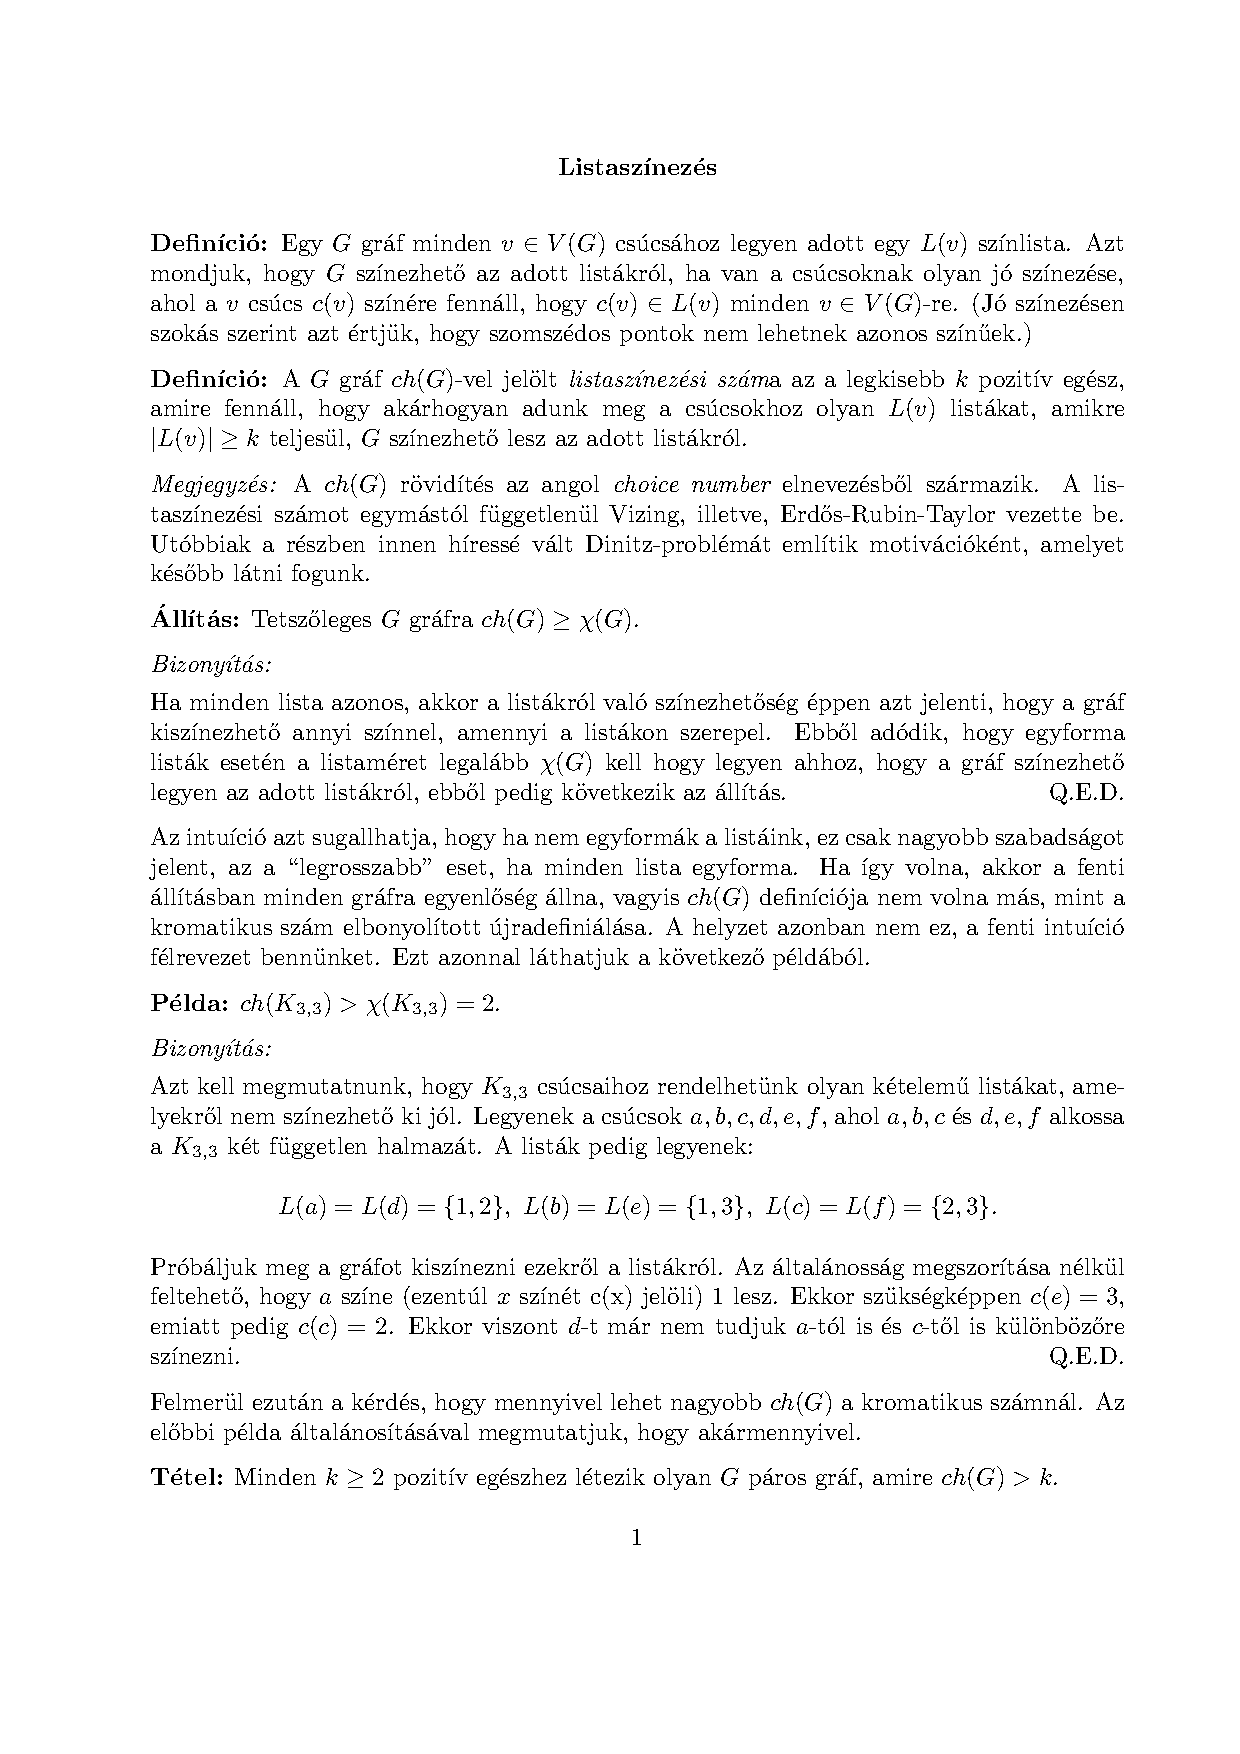
\includepdf[pages=-]{chapters/09_listaszinezes_simonyi}

\chapter{Lovász-Kneser tétel és Greene féle bizonyítása. Dolnyikov tétele és annak magyarázata, hogy miért következik belőle a Lovász-Kneser tétel.}

\begin{notation}
  $S^d: d$ dimenziós gömb felszíne.
\end{notation}

\begin{thm} Borsuk-Ulan tétel:
  Ha $f: S^d \rightarrow \RR^d$ folytonos függvény, akkor $\exists x \in S^d$, amire $f(x) = f(-x)$.
\end{thm}

\begin{dfn}
  Egy $U$ halmaz nyílt, ha $\forall x \in U$-nak $\exists$ olyan kis környezete, ami teljesen $U$-ban van. Egy halmaz zárt, ha a komplementere nyílt.
\end{dfn}

\begin{thm} Lusternik-Schnirel'mann tétel:
  \begin{enumerate}
    \item Legyenek $A_1, A_2, \dots, A_m \subseteq S^d$ zárt halmazok, melyekre
    $\overset{m}{\underset{i=1}{\text{\LARGE $\cup$}}} A_i = S^d$ és $\forall i, x \in A_i \Rightarrow -x \not \in A_i$. Ekkor $m \geq d + 2$.
    \item ugyanez, ha $A_i$ nyílt
    \item ugyanez, ha $A_i$ nyílt vagy zárt
  \end{enumerate}
\end{thm}

Bizonyítás (zárt eset, Borsuk-Ulan tétel alapján):
Tekintsük $S^d$-nek egy $A_1, \dots, A_{d+1}$ halmazokkal való fedését, ahol $\forall A_i$ zárt $(\overset{d+1}{\underset{i=1}{\text{\LARGE $\cup$}}} A_i = S^d)$.

$f: x \rightarrow (\text{dist}(x, A_1), \text{dist}(x, A_2), \dots, \text{dist}(x, A_d))$.

Ez egy folytonos $S^d \rightarrow \RR^d$ függvény $\underbrace{\Rightarrow}_{\text{BU tétel}} \exists x_0 \in S^d: f(x) = f(-x)$.

Ha $\exists i$, hogy $x_0 i.$ koordinátája nulla, akkor $x_0, -x_0 \in A_i$. Ha $\not \exists$ ilyen $i$, akkor $x_0, -x_0 \in A_{d+1}$. Vagyis mindenképpen van egy antipodális pontpárt tartalmazó $A_i$.
\QED

\begin{dfn}
  $n, k \in \NN, k < \frac{n}{2}$ esetén az $n, k$ paraméterű $KG(n, k)$ Kneser gráf a következő:

  \begin{flalign}
    V(KG(n,k)) &= \binom{[n]}{k} &\\
    E(KG(n,k)) &= \{AB: A,B \in \binom{[n]}{k}, A \cap B = \emptyset\}
  \end{flalign}
\end{dfn}

\begin{thm} Lovász-Kneser tétel:
  $\chi(KG(n, k)) = n - 2k + 2$
\end{thm}

Bizonyítás (Greene):
Tekintsük $S^{n - 2k + 1}$-et és rajta $n$ pontot általános helyzetben, azaz semelyik $n - 2k + 2$ nem esik közös főkörre.

Vegyük $KG(n, k)$ egy jó színezését $m$ színnel, és definiáljuk az $A_i, \dots, A_m \subseteq S^{n-2k+1}$ nyílt halmazokat úgy, hogy $x \in A_i$, ha az $x$ középpontú nyílt félgömb tartalmaz olyan $k$ pontot, hogy az azoknak megfelelő $K(n, k)$-beli csúcspont az adott színezésben $i$ színű.

\medskip

$\forall A_i$ nyílt, és antipodális pontpármentes, hiszen ha $x \in A_i$ és $-x \in A_i$, akkor $H(x)$ és $H(-x)$ tartalmaz két diszjunkt $k$-ast, ami $KG(n,k)$ két összekötött csúcspont, és mindkettő $i$ színű \Lightning.

\medskip

$B := S^{n-2k+1} \backslash \overset{n}{\underset{i=1}{\text{\LARGE $\cup$}}} A_i$, \hspace{1em} $B$ zárt.

\medskip

$x \in B \Rightarrow -x \not \in B$, mert ha $x \in B$, akkor $H(x)$ legfeljebb $k-1$ pontot tartalmaz (ha lenne rajta $k$ pont, akkor $x$ valamelyik $A_i$-nek része lenne), és ugyanígy ha $-x \in B$, akkor $H(-x)$ legfeljebb $k-1$ pontot tartalmaz. Emiatt ha $x, -x \in B$, akkor a $H(x)$ és $H(-x)$-et elválasztó főkörön legalább $n-2(k-1)=n-2k+2$ pont van. \Lightning$.

\medskip

A Lusternik-Schnirel'mann tétel (nyílt és zárt vegyes változata) miatt:

\begin{align}
m + 1 &\geq n - 2k + 1 + 2 \\
m &\geq n - 2k + 2
\end{align}

\QED

\begin{dfn}
  Legyen $\HH=(V, E)$ egy hipergráf. $cd_2(\HH) = \min\{|u| : u \subseteq V, \chi(\HH \backslash u) \leq 2\}
\end{dfn}

\begin{dfn}
  Egy $\FF$ halmazrendszerhez rendelt általánosított Kneser-gráf, $KG(\FF)$ a következő:

  \begin{flalign}
    V(KG(n,k)) &= \FF &\\
    E(KG(n,k)) &= \{AB: A,B \in \FF, A \cap B = \emptyset\}
  \end{flalign}
\end{dfn}

\begin{thm} Dolnyikov tétel:
  $\forall \FF \subseteq 2^{[n]}: \chi(KG(\FF)) = cd_2(\FF)$
\end{thm}

Ez általánosítása a Lovász-Knézer tételnek:
$\FF := \binom{[n]}{k}, cd_2(\FF) = n-2(k-1) = n-2k+2$ (ugyanis két megmaradó színosztály egyikében sem lehet maradhat $k$ pont, szóval kevesebb pont elhagyása nem elég, de ha mindkét színosztályban $k-1$ pont marad, akkor a gráf már kettő kromatikus). Vagyis $\chi(KG(\FF)) = cd_2(\FF) = n-2k+2$.



\printbibliography

\label{page:last}

\end{document}

%%% Local Variables:
%%% mode: latex
%%% TeX-master: nil
%%% End:
